% intro


\newpage
\section{Finite Element Method}%
\label{sec:finite_element_method}


\begin{frame}{}
        \begin{block}{Finite Element Methods!}
            \begin{itemize}
                \item To simplify will I only consider Poisson equation $ \Delta u =f $
                    \begin{itemize}
                        \item However, same ideas applies to Navier-Stokes and Cahn-Hilliard
                    \end{itemize}
                \item But to tell the story we need to do math
                    \begin{itemize}
                        \item Notation, inverse inequalities, variational forms, domains etc
                        \item \textbf{I will skip a lot of details,} but still promote the main ideas.
                    \end{itemize}
            \end{itemize}
        \end{block}
\end{frame}

\begin{frame}{}
        \begin{block}{We start with finite difference}
            \begin{itemize}
                \item Then we gradually introduce flaws and problems!
            \end{itemize}
        \end{block}
\end{frame}

\begin{frame}{Poisson Problem}
    Let us define the physical domain $\Omega  \subset \mathbb{R} ^{2}$ and the scalar functions $f: \Omega  \to \mathbb{R}$ and $g: \Omega  \to \mathbb{R} $.
        \begin{block}{Poisson Problem}
  We define the strong formulation of the Possion problem to find a scalar solution
 $u:\Omega  \to \mathbb{R} $ s.t. \[
\begin{split}
    -\Delta u &= f \quad  \text{in }\Omega  \\
     u &= g  \quad \text{on } \Gamma      \\
\end{split} .
\]
        \end{block}
\end{frame}

\begin{frame}{}
        \begin{block}{Finite difference approach}
            \begin{itemize}
                \item Taylor expansion in $y$ and $x$ direction. \[
                        \begin{split}
                \Delta u & = u_{xx} + u_{yy} \\
                & \approx  \frac{u( x-h, y) - 2u( x,y) + u( x +h,y)   }{h^2} + \frac{u( x, y-h) - 2u( x,y) + u( x,y +h)   }{h^2}
                        \end{split}
                \]
            \item Works very well for perfectly square domains
                \begin{figure}
                    \centering
                    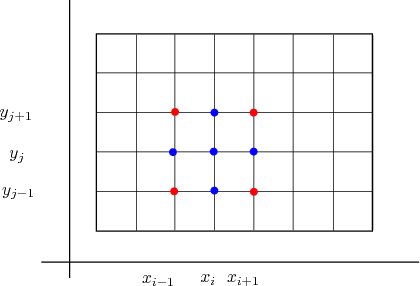
\includegraphics[width=0.35 \textwidth]{figures/fdm.png}
                \end{figure}
            \end{itemize}
        \end{block}
\end{frame}

\begin{frame}{}
        \begin{block}{Finite difference approach}
            \begin{itemize}
            \item Can be very messy for unstructured mesh!
                \begin{figure}
                    \centering
                    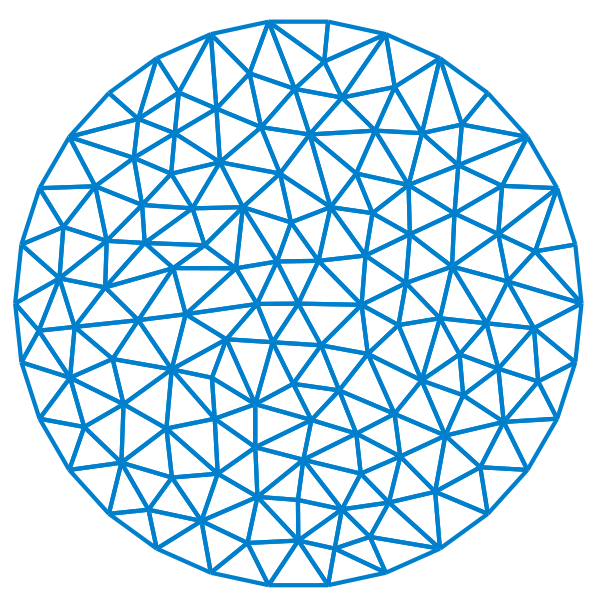
\includegraphics[width=0.35 \textwidth]{figures/triangulation.png}
                \end{figure}
            \item It does exists methods for handling nodes on these domains.
                \begin{itemize}
                    \item The implementation can be very messy
                    \item Does not scale that well as far as I know.
                \end{itemize}
            \end{itemize}
        \end{block}
\end{frame}


\begin{frame}{Finite element method}
        \begin{block}{Finite element approach for triangulations}
            \begin{enumerate}
                \item We want to write the problem on a equivalent integral form.
                \item Introduce so-called test functions space
                \item Introduce a discrete polynomial space as an approximation space.
            \end{enumerate}
        \end{block}
\end{frame}

\begin{frame}{Finite element method}

        \begin{block}{Let us introduce some notation}
            \begin{itemize}
                \item
                 Function spaces
                    \begin{equation*}
                        \begin{split}
                        L^{2}( \Omega  ) & = \left\{ f: \Omega \mapsto \mathbb{R}  \mid \int_{\Omega }^{} \left\lvert f \right\rvert ^{2} d \Omega  < \infty  \right\} \\
                        H^{1}( \Omega  ) & = \left\{ u \in L^{2}\left( \Omega  \right)  \text{ and }  \nabla  u \in L^{2}\left( \Omega  \right)   \right\}.
                        \end{split}
                    .\end{equation*}

                \item Essentially is $L^2( \Omega ) $ the space of all integrable functions.
                    \begin{itemize}
                        \item \textbf{Example:} $ \int_{-1}^{1} (\frac{1}{x}) dx  $ is not $L^2(\left[ -1,1 \right] )$  integrable. \\
                        \item \textbf{Example:} $ \int_{2}^{3} (\frac{1}{x}) dx  $ is $L^2(\left[ 2,3 \right] )$  integrable. \\
                    \end{itemize}


                \item $H^{1}( \Omega )$ is the space off all functions where both the function and its first derivative is integrable.
            \end{itemize}

        \end{block}
\end{frame}


\begin{frame}{Finite element method}

        \begin{block}{Norms and inner products}
            \begin{itemize}
                \item For $u ,v \in L^2( \Omega )  $ we define  \[
                        \begin{split}
\| u \|_{  \Omega   }^{  } & = \| u \|_{ L^{2}\left( \Omega  \right)  }^{  }   = \left( \int_{\Omega }^{} \left\lvert u \right\rvert ^{2} dx  \right) ^{\frac{1}{2}} \\
\left( u,v \right) _{\Omega } & = \left( u,v \right) _{L^2\left( \Omega  \right) } = \int_{\Omega }^{} u  v dx. \\
                        \end{split}
                    \]
                \item  For $u,v \in H^1( \Omega ) $ we define \[
                    \begin{split}
\| u \|_{ H^{1}\left( \Omega  \right)  }^{  }  & =  \| u \|_{ \Omega } +\| \nabla u \|_{ \Omega }    , \\
\left( u,v \right) _{H^{1}( \Omega )  } & = \left( u,v \right) _{\Omega  } + \left( \nabla u, \nabla v \right) _{\Omega  }
                    \end{split} .
                    \]
            \end{itemize}

        \end{block}

\end{frame}


\begin{frame}{Finite element method}
        \begin{block}{Writing the Poission problem on an integral form   }
            \begin{enumerate}
                \item We extent the definitions for the boundary conditions s.t.
                    \begin{itemize}
                        \item $H^{1}_{0} = \left\{ v \in H^{1 }( \Omega )   \mid  v = 0 \text{ on } \Gamma   \right\} $
                        \item  $V_{g} = \left\{ v \in H^{1 }( \Omega )   \mid  u = g \text{ on }  \Gamma   \right\} $
                    \end{itemize}
                    Notice that the boundary conditions is built in to the space!
                \item Let $u \in V_{g}$. If we multiply with a so-called test function $v \in H^{1}_{0}( \Omega ) $ and apply Greens theorem we get
                    \[
                - \int_\Omega  \Delta u v dx  = \int_\Omega  \nabla u \nabla v dx - \int_\Gamma \partial _{n} u v dx  =  \int_\Omega  \nabla u \nabla v dx
                    \]

                    We will use the following compact notation:
                    \[
                -( \Delta u, v) _{\Omega } = ( \nabla u, \nabla v)_{\Omega} - (\partial _{n} u, v )_{\Gamma }  =  ( \nabla u, \nabla v)_{\Omega}
                \]

            \end{enumerate}
        \end{block}
\end{frame}

\begin{frame}{Finite element method}
        \begin{block}{Writing the Poission problem on an integral form  }
             Let us denote a bilinear form and a linear form \[
            a( u,v)  := ( \nabla u,\nabla v)_{\Omega } \text{ and }  \quad l ( v) := ( f,v) _{\Omega  }
            \]
            The weak formulation of the Poisson problem is to find a $u \in V_{g}$ s.t. \[
            a( u,v) = l ( v) \quad  \forall v  \in  H^{1}_{0}( \Omega  )
            \]

        \end{block}

        How can we discretize the following function spaces?
\end{frame}

\begin{frame}{Abstract definition of a finite element}
    \begin{block}{}
    We define a element as the triple $(T, \mathcal{P}, \Sigma )$ where,
    \begin{itemize}
        \item $T$ is an triangle
        \item $\mathcal{P}^{k}( T)   $ is a finite polynomial basis $\left\{ \phi  \right\}_{i}^{n} $  of dimension $k$, also known as shape functions.
        \item $\Sigma $ is the dual of $\mathcal{P}^{k}( T)  $, that is, the set of linear forms $\left\{ \sigma _{i} \right\}_{i}^{n} $ with the mapping,
            \[
            \sigma _{i}:  \mathcal{P}^{k}( T) \to \mathbb{R} \quad  \text{ such that  } \quad   \sigma _{i}( \phi _{j})  = \delta _{ij}
            \]
            Also contains the DOFs or the coefficients in the polynom!
    \end{itemize}
    \end{block}

    \textbf{Example:} For $k=1$ the DOF in a triangle is one coefficient per mesh node, i.e., number of DOFs is $n = 3$.


\end{frame}

\begin{frame}{Finite element method}
    The absolute key idea of the finite element methods is the following; \\
    \begin{itemize}
        \item \textbf{ The goal is to approximate the (infinite dimensial) function space $H^{1}( \Omega ) $ with a finite dimensional polynomial space $\mathcal{P}^{k}( \Omega ) = span  \left\{ \phi_{1}, \ldots, \phi _{N}  \right\} $ of order $k$  }
    \end{itemize}

\end{frame}

\begin{frame}{Finite element method}
    To solve the Poisson problem using FEM we have the following discrete problem;

    \begin{block}{ Discrete Poisson problem }
    We want to find an $u_{h} \in V_{h} := \mathcal{P}^{k}( \Omega )  $ s.t. \[
    a( u_{h}, v_{h}) = l ( v_{h}) \quad  \forall v_{h} \in V_{h}
    \]
    \end{block}

\end{frame}

\begin{frame}{Finite element method}

    \begin{block}{ Constructing the linear system  }
        \begin{itemize}
            \item Since $v_{h}, u_{h} \in V_{h} := \mathcal{P}^{k}( \Omega )  $ can we write $u_{h} = \sum_{i=0}^{N} U_{i} \phi _{i} $ and $v_{h} = \sum_{i=0}^{N} U_{i} \phi _{i} $ with coefficients $\left\{ U_{i} \right\}_{i=0} ^{N} $ and $\left\{ V_{i} \right\}_{i=0} ^{N} $.
        \item Let us define a matrix $\left[ \mathcal{A}  \right] _{ji} = a( \phi_{i}, \phi _{j} ) $ and $\left[ F \right] _{j} = l( \phi _{j})   $.
        \end{itemize}
    \end{block}
    Thus, we have \[
    \sum_{i,j}^{N} V_{j} U_{i}\ a( \phi_{j}, \phi _{i} ) =  \sum_{j}^{N} V_{j}\ l(\phi _{j})     .
    \]
    Hence, we have the following equivalent linear system, that is \[
    \mathcal{A} U = F.
    \]
\end{frame}

\begin{frame}{Energy norm}

   We will now show requirements for uniqueness of numerical solution, but we need the so-called energy norm.

   \begin{block}{  }
    The energy norm  is denoted by  \[
    \| v \|_{a  }^{ 2 } = a( v,v)
    \]
    \end{block}



\end{frame}

\begin{frame}{Requirements for a well-posed problem}
    \begin{theorem}[ The (discrete) Lax-Milgram Theorem]
        Assume we have a general the bilinear form  $a_{h}: V_{h} \times V_{h} \to \mathbb{R}  $ and a bounded linear form $l_{h}: V_{h} \to \mathbb{R} $. If there exists some constants $C_{1} >0$ and $C_{2} >0$  such that;
        \begin{enumerate}
            \item The bilinear form is bounded,
                \[
                      \abs{a_{h}( v,w)  }    \le C_{1} \| v \|_{a_{h}  }^{  }  \| w \|_{a_{h}  }^{  } \quad \forall v,w  \in V_{h}.
                \]
            \item The bilinear form is coercive (one-to-one), \[
           a_{h}( v,v) \ge  C_{2} \| v \|_{ a_{h} }^{  2} \quad \forall v \in V_{h}.
            \]
        \end{enumerate}
        then it exists a unique discrete solution $u \in V_{h}$ s.t. \[
        a_{h}( u,v)  = l_{h}( v) \quad  \forall v \in V_{h}
        \]
    \end{theorem}


\end{frame}

\begin{frame}{Why is a well-posed problem so interesting?}
    \begin{block}{ Consequences of Lax Milgram }
    \begin{enumerate}
        \item The solution is accurate and reliable.
        \item The discrete problem converges when $h\to 0$
        \item Does not exists infinite solutions
        \item The problem is stable respect to small perturbation.
    \end{enumerate}

    \end{block}
    \begin{block}{Conclusion}
        \begin{itemize}
            \item Lax-Milgram very useful and rigour tool when developing new FEM schemes.
            \item Still hard to apply directly nonlinear problems, but we use it as a basis on simplified problems before we introduce nonlinear terms.
                \begin{enumerate}
                    \item Stokes equation vs Navier Stokes equation
                    \item Biharmonic equation vs Chan Hilliard equation
                \end{enumerate}
        \end{itemize}
    \end{block}

\end{frame}




